%%%%%%%%%%%%%%%%%%%%%%%%%%%
% PREAMBOLO DEL DOCUMENTO %
%%%%%%%%%%%%%%%%%%%%%%%%%%%
\documentclass[a4paper,11pt,oneside,top=3cm,bottom=3cm,left=3.5cm,right=3.5cm,openright,reqno,table]{book}

% openany - fa iniziare i capitoli direttamente nella pagina successiva
% openright - fa iniziare i capitoli nella prima pagina destra disponibile 
% fleqn  - allinea le formule a sinistra anzichè centrarle
% leqno - dispone la numerazione delle formule sulla sinistra o destra
% reqno - dispone la numerazione delle formule sulla destra
%
\usepackage{packages}
% Per non appesantire troppo questo file
% quasi tutti i pacchetti usati sono salvati in packages.sty
%
\linespread{1.5}
% Per avere la parola BOZZA scritta su tutte le pagine

% funziona solo in modalità PS
% Invece per i PDF ho risolto così:
% pdftk tesi.pdf background bozza.pdf output tesi_bozza.pdf
%
%%%%%%%%%%%%%%%%%%%%%%%%%%%%%%%%%
%   DOCUMENTO VERO E PROPRIO    %
%%%%%%%%%%%%%%%%%%%%%%%%%%%%%%%%%
\begin{document}
% FRONTESPIZIO %
\begin{titlepage}
\changepage{}{}{}{-7.5 mm}{}{}{}{}{}
% parametri per cambiare le dimensioni di una singola pagina in ordine:
% {textheight}{textwidth}{evensidemargin}{oddsidemargin}{columnsep}
% {topmargin}{headheight}{headsep}{footskip}
% se voglio centrare la pagina devo mettere bindingoffset/2
% i primi 5 parametri posso usarli con \changetext


\begin{center}

\includegraphics [width=.15\columnwidth, angle=0]{unisa}\\ % height
\vspace{0.5cm}
{\LARGE \scshape Università degli Studi di Salerno}\\
\vspace{0.5cm}
{\Large Dipartimento di Informatica}\\
\vspace{0.1cm}
{\large Corso di Laurea Magistrale in Informatica}\\
\vspace{1.5cm}
{\Large \scshape Corso di Penetration Testing\\ and Ethical Hacking} \\
\vspace{4cm}
{\Huge \bfseries De-ICE S1.140} \\
\vspace{5cm}

\begin{minipage}[t]{7cm}
\flushleft
\textsc{Studente}

Lorenzo Criscuolo \\
Matricola: 0522501268
\end{minipage}
\hfill
\begin{minipage}[t]{7cm}
\flushright
\textsc{Docente}

Prof. \textbf{Arcangelo Castiglione} \\
{\small Università degli studi di Salerno} \\[0.25cm]
\end{minipage}

\vspace{3cm}

{\small Anno Accademico 2022-2023} %\\
%

%
\end{center}

\end{titlepage}
%

\frontmatter
% quello che segue è in numerazione romana e i capitoli non verranno numerati
% se non si vuole che compaia il numero di pagina basta usare il comando:
%\nonumber

% SOMMARIO %
\cleardoublepage
\include{frontmatter/sommario}
% INDICI %
\phantomsection
\addcontentsline{toc}{chapter}{Indice}
\tableofcontents
% Il simbolo * serve per evitare che comapaia nell'indice
\clearpage
%\listoffigures
%\clearpage
%\listoftables

\mainmatter
% quello che segue sarà in numerazione araba e i capitoli verranno numerati
%\part{Studio iniziale}
% CAPITOLI
\phantomsection
%\addcontentsline{toc}{chapter}{Introduzione}
\chapter{Introduzione}
\markboth{Introduzione}{}
Il presente documento ha lo scopo di illustrare passo-passo tutte le attività svolte durante il progetto del corso di "\emph{Penetration Testing and Ethical Hacking}". Per lo svolgimento dello stesso è stato necessario scegliere un asset da analizzare e, dunque, è stata scelta una macchina virtuale vulnerabile by-design identificata con il nome \textbf{De-ICE S1.140} e indicizzata al seguente indirizzo: \url{https://www.vulnhub.com/entry/de-ice-s1140,57/}.

L'intera attività progettuale sarà suddivisa in fasi, in modo da emulare nel modo più preciso possibile il lavoro svolto da un hacker etico e per contestualizzare al meglio ogni passo eseguito durante il processo. Le fasi in cui sarà suddivisa l'attività sono:
\begin{itemize}
    \item \textbf{Target Scoping}: in questa fase vengono presi accordi con il proprietario dell'asset da analizzare, definendo limiti riguardo host da analizzare, indirizzi, ecc. e definendo le metodologie da applicare;
    \item \textbf{Information Gathering}: in questa fase si impiegano varie tecniche e strumenti con lo scopo di raccogliere quante più informazioni possibile riguardo l'asset come personale afferente all'organizzazione, indirizzi e-mail, software utilizzati nell'organizzazione (utili per eventuale attività di Social Engineering), infrastruttura di rete, domini DNS e, in generale, ogni informazione che può essere utile per le fasi successive del processo;
    \item \textbf{Target Discovery}: in questa fase vengono impiegate strategie e strumenti attivi e passivi per scansionare la rete (o le sottoreti) per identificare le macchine effettivamente attive nell'asset da analizzare e l'OS che utilizzano;
    \item \textbf{Target Enumeration}: in questa fase viene eseguita una scansione a livello di servizi offerti sulle macchine identificate con lo scopo di capire, appunto, quali servizi vengono offerti e le versioni di questi;
    \item \textbf{Vulnerability mapping}: in questa fase si cerca di capire quali sono le eventuali vulnerabilità di cui sono affette le versioni dei servizi identificati nella fase precedente;
    \item (\textbf{\emph{CONTINUA}})
\end{itemize}


\section{Ambiente utilizzato}
Essendo che l'asset da analizzare è una \emph{macchina virtuale} dovrà essere necessariamente utilizzato un \emph{ambiente di virtualizzazione} appropriato.
Per questa ragione, è stato utilizzato \textbf{Oracle VM VirtualBox 7.0.8} per creare un \emph{ambiente di virtualizzazione} sul quale poi effettuare l'intero processo. Oltre a creare l'ambiente di esecuzione della macchina è stato necessario eseguire un altro passo, ovvero la \emph{creazione di una rete} con la quale poi essere in grado di comunicare con l'asset stesso. Fortunatamente, \emph{VirtualBox} rende disponibile la funzionalità di \emph{NAT} e, infatti, in maniera molto semplice è possibile creare una \textbf{rete NAT ad-hoc} sulla quale collegare l'asset da analizzare (ed eventuali altre macchine).
Per realizzare questa rete \emph{NAT}, tutto quello che bisogna fare è:
\begin{enumerate}
    \item Aprire il pannello degli strumenti di VirtualBox;
    \item Selezionare il sotto-menù rete;
    \item All'interno della pagina, selezionare il pannello "Reti con NAT";
    \item Cliccare il pulsante per la creazione di una nuova rete ed impostare i parametri desiderati.
\end{enumerate}
Per essere conformi alle istruzioni fornite dal docente durante le lezioni riguardo la definizione dell'ambiente, i parametri della rete saranno i seguenti: 
\begin{itemize}
    \item \textbf{Nome della rete}: Corso
    \item \textbf{Spazio di indirizzamento}: 10.0.2.0/24
\end{itemize}

Come ultimo passo, per fare in modo che l'asset (e altre eventuali macchine) utilizzi questa rete creata \emph{ad-hoc}, basta aprire le impostazioni di rete della macchina e impostare come rete da utilizzare (nel rispettivo menù a riguardo) la rete NAT appena creata identificata dal nome scelto in precedenza.

Il risultato che si ottiene quando si configurano in questo modo l'asset e VirtualBox è il seguente schema di rete:

\begin{figure}[h]
    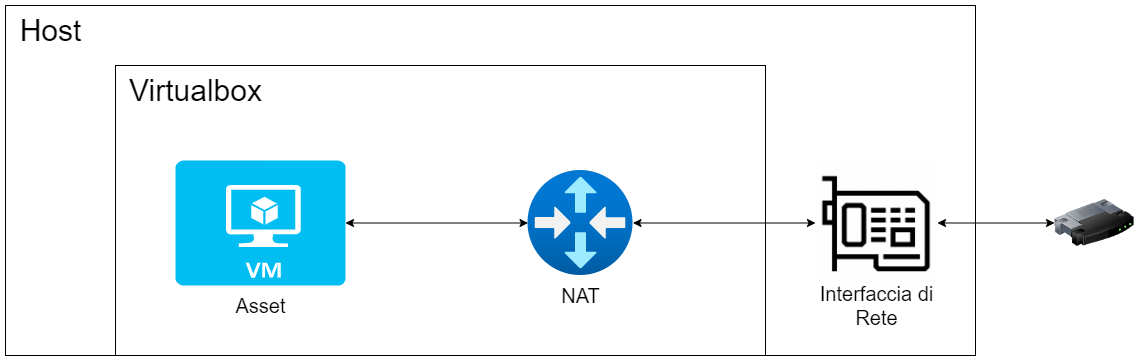
\includegraphics[scale=0.3]{capitoli/figure/schema-rete-nat-solo-asset.png}
    \caption{Infrastruttura di rete}
\end{figure}


\section{Strumenti utilizzati}
Per proseguire con l'analisi dell'asset, è necessario ottenere strumenti appositi che permettono di realizzare scansioni, mapping di vulnerabilità, ecc. Visto che, come già detto in precedenza, l'asset è una \emph{macchina virtuale} che sarà eseguita in un \emph{ambiente di virtualizzazione} e all'interno di una \emph{rete virtuale con NAT}, il modo più semplice per analizzare l'asset è quella di utilizzare una macchina virtuale realizzata apposta per questo scopo. A tal proposito, si è scelto di utilizzare una macchina virtuale molto popolare chiamata \textbf{Kali Linux} (in particolare la versione di riferimento \textbf{2023.1}) che viene distribuito con una suite di strumenti pronti all'uso per effettuare attività di Penetration Testing, Digital Forensics e altre simili. A questo punto, essendo che anche \textbf{Kali Linux} è una macchina virtuale che viene eseguita all'interno di \emph{VirtualBox}, verrà configurata anch'essa in modo tale che si colleghi alla \emph{rete con NAT} creata in precedenza. Otteniamo così il seguente schema:

\begin{figure}[h]
    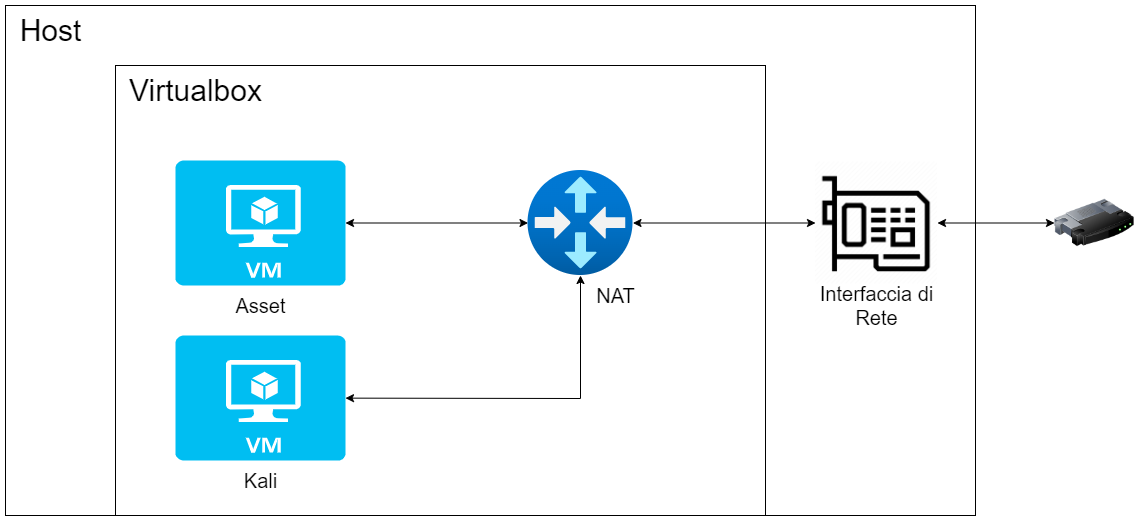
\includegraphics[scale=0.25]{capitoli/figure/schema-rete-nat-kali.png}
    \caption{Infrastruttura di rete con Kali}
\end{figure}
\chapter{Pre-Exploitation}
\markboth{Pre-Exploitation}{}

\section{Target Scoping}
In questa fase bisogna stipulare un accordo tra le parti (responsabile dell'asset e pentester) in modo da definire vincoli, limiti, responsabilità legali in caso di eventuali problemi, accordo di non divulgazione, ecc. Tuttavia, possiamo fare le seguenti osservazioni:

\begin{itemize}
    \item L'asset da analizzare è pubblicamente disponibile e realizzato appositamente per essere analizzato, ossia vulnerabile by-design;
    \item Tutta l'analisi avviene in un ambiente virtualizzato all'interno della macchina in possesso al Penetration Tester;
    \item Lo scopo dell'analisi è puramente didattico, in quanto realizzato in un contesto universitario e, più precisamente, come progetto del corso "Penetration Testing and Ethical Hacking";
    \item Tutti gli strumenti utilizzati e le fonti consultate sono pubblicamente disponibili e accessibili o, in generale, sono accessibili tramite piani gratuiti e quindi senza costi da sostenere.
\end{itemize}

In conclusione, come si può notare dalle precedenti osservazioni, questa fase può essere tranquillamente saltata visto che non ci sono parti con cui prendere accordi e non possono esserci problematiche di tipo legale dal momento che l'ambiente è totalmente simulato.

\section{Information Gathering}
Durante questa fase, l'obiettivo è quello di trovare più informazioni possibili riguardo l'asset scelto e, essendo che l'asset è una macchina virtuale che viene eseguita in un \emph{ambiente virtualizzato} e in una \emph{rete con NAT virtuale} (come illustrato nell'introduzione), si eviteranno fonti e tool che raccolgono informazioni riguardo persone afferenti all'organizzazione dell'asset, indirizzi e-mail, analisi di record DNS, informazioni di routing e così via. A questo punto, l'unica tecnica che ha senso utilizzare (e che è stata effettivamente utilizzata) è \textbf{OSINT} (\emph{Open Source INTelligence}), con cui si cercherà di individuare nomi utente, password, indirizzo IP, ecc. Tutto questo, ovviamente, evitando di consultare fonti dove sono presenti Walktrough e guide per evitare di vanificare il contributo didattico del processo.

Come primo passo, è stata consultata la pagina di Vulnhub sulla quale sono riportate varie informazioni riguardo la macchina virtuale scelta "\textbf{De-ICE S1.140}" e,
all'interno della pagina, sono state trovate le seguenti informazioni:
\begin{itemize}
    \item Informazioni riguardo il \textbf{rilascio}, ovvero autore, data, sorgente e valore hash della macchina. Queste informazioni, tuttavia, non sembrano essere utili per il processo;
    \item Una \textbf{descrizione} molto ad alto livello della macchina. Anche qui non viene rilasciata alcuna informazione utile come servizi esposti dalla macchina o credenziali di accesso alla macchina (anche non privilegiate). Infatti, attualmente, se avviamo la macchina non possiamo fare nulla tramite \emph{interazione diretta} in quanto \textbf{non abbiamo nessuna credenziale di accesso};
    \item Informazioni riguardo la configurazione dell'\textbf{indirizzo di rete}. Questa informazione è molto utile perché ci rivela che la macchina \textbf{non è configurata per lavorare con un indirizzo IP specifico} ma lo ottiene in maniera automatica grazie al servizio \textbf{DHCP}. Questo ci fa subito capire che all'interno della rete con NAT non avremo problemi di indirizzamento ma, sfortunatamente, questo significa che non conosciamo apriori l'indirizzo della macchina (sappiamo solo che sarà all'interno della rete \emph{10.0.2.0/24}) ma dovremo ricavarcelo in maniera indiretta visto che \emph{VirtualBox} non fornisce un metodo diretto di ottenimento degli indirizzi IP e \textbf{non abbiamo accesso alla macchina};
    \item Informazioni riguardo il \textbf{sistema operativo}. Altra informazione molto utile in quanto adesso sappiamo che l'asset è un sistema Linux e questo ci permetterà di risparmiare tempo in fasi avanzate perché possiamo restringere il campo delle scansioni solo a sistemi Linux, escludendo tutti gli altri. Tuttavia, non sappiamo ancora la versione precisa del kernel e quindi dobbiamo ricavarla successivamente;
\end{itemize}

Andando più a fondo nella pagina si può ricavare l'indirizzo del \textbf{sito web del creatore} dell'asset e il \textbf{link di download della macchina} ma, sfortunatamente, entrambi i link \textbf{non sono più attivi}. Consultando il motore di ricerca Google, semplicemente ricercando il nome dell'organizzazione trovato sulla pagina, è possibile risalire al rispettivo account Twitter e si nota che quest'ultimo non è attivo all'incirca dal 2020. Per questa ragione, è sembrato opportuno accedere al servizio \emph{WaybackMachine} offerto da \textbf{Archive.org} per visitare versioni precedenti del sito dell'organizzazione nella speranza di trovare altre informazioni utili. Fortunatamente, grazie a questo servizio è stato possibile accedere ad uno \emph{snapshot} risalente al 2021 dal quale è stato anche possibile effettuare il download della macchina. Ad ogni modo, anche accedendo al sito e, in particolare, alla pagina di download, non sono state trovate informazioni rilevanti come credenziali, porte aperte, schemi di naming, ecc.

\section{Target Discovery}
In questa fase si avvieranno entrambe le macchine e si procederà con la scansione della rete \emph{Corso}, con lo scopo di trovare tutte le macchine attive all'interno della stessa. Ovviamente ci aspettiamo di trovare solo la macchina \textbf{De-ICE S1.140} e la macchina \textbf{Kali} per come abbiamo impostato l'ambiente.

\subsection{Esecuzione di \texttt{ifconfig}}
Prima di cominciare con la scansione effettiva della rete, dobbiamo capire qual è l'indirizzo della macchina \textbf{Kali} in modo da escludere il suo IP da successive scansioni più approfondite. Per ottenere questa informazione ci basta semplicemente lanciare il comando \texttt{ifconfig} e,una volta lanciato questo comando, otteniamo il seguente output:
\begin{figure}[h]
    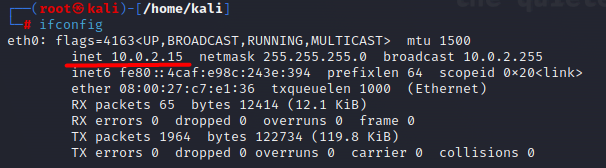
\includegraphics[width=0.8\textwidth]{capitoli/figure/ifconfig-kali.png}
    \centering
    \caption{Esecuzione di \texttt{ifconfig} su Kali}
    \label{fig:ifconfig}
\end{figure}

Come possiamo notare dall'output, l'indirizzo di Kali è \emph{10.0.2.15} e, adesso che lo conosciamo, possiamo cominciare con la scansione della rete.
\subsection{Scansione con \texttt{nmap}}
Il primo strumento utilizzato per la scansione è \texttt{nmap}, un potentissimo strumento di scansione che tornerà molto utile anche nelle successive fasi. In particolare, tra le varie tipologie che offre \texttt{nmap}, permette anche di eseguire una scansione di tipo \textbf{ICMP} (detta \emph{ping scan}) su una determinata sottorete presa in input. Con questa scansione, \texttt{nmap} invierà a tutti gli indirizzi specificati dei pacchetti \emph{ICMP Echo Request} e, se prima dello scadere di un timeout prefissato, riceve da un host un pacchetto \emph{ICMP Echo Reply}, \texttt{nmap} capirà che l’host è attivo e risponde altrimenti marcherà quell’indirizzo come non attivo. Per eseguire una \emph{ping scan} sulla rete \emph{Corso} basta lanciare il seguente comando:

\begin{lstlisting}[language=bash]
    nmap -sP 10.0.2.0/24
\end{lstlisting}

Una volta lanciato questo comando, possiamo osservare il seguente output:
\begin{figure}[h]
    \centering
    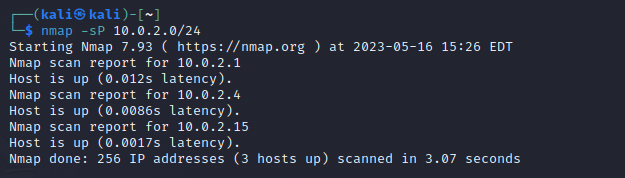
\includegraphics[width=0.8\textwidth]{capitoli/figure/discovery-nmap.png}
    \caption{Risultato della \emph{ping scan} con \texttt{nmap}}
    \label{fig:nmap-ping-scan}
\end{figure}

Il primo dato che dovrebbe risaltare è che il numero degli host attivi sulla rete è 3, e non 2 come in realtà ci si aspettava dalla configurazione realizzata. Tuttavia, come specificato a lezione e approfondito anche nella documentazione di \emph{VirtualBox}, all'interno della rete saranno presenti uno o più host "\emph{fittizi}" che sono necessari allo stesso \emph{VirtualBox} per realizzare la stessa \emph{rete con NAT}. Questi host di solito hanno sempre i primi indirizzi assegnabili, quindi è lecito pensare che l'host con indirizzo \emph{10.0.2.1} sia proprio l'host interno di \emph{VirtualBox} e che l'host con indirizzo \emph{10.0.2.4} sia il nostro asset. Per quanto riguarda \emph{10.0.2.15}, in realtà già lo conosciamo dal comando lanciato prima e sappiamo per certo che è proprio l'indirizzo della macchina \textbf{Kali}.

\subsection{Scansione con \texttt{arp-scan}}
Grazie ad \texttt{nmap} conosciamo gli indirizzi IP degli host attivi all'interno della rete, però in seguito potremmo essere interessati anche agli indirizzi \emph{MAC} corrispondenti. Questo perchè l'infrastruttura di rete è composta da un solo \emph{router virtuale} al quale si collegano tutti gli host (come indicato anche nella Figura \ref{fig:infrastruttura-kali}) e, per questa ragione, è possibile utilizzare anche il protocollo \textbf{ARP} essendo una rete locale. A tal proposito, è stato utilizzato il tool \texttt{arp-scan} che, sfruttando proprio il protocollo \textbf{ARP}, è in grado di ottenere gli indirizzi \emph{MAC} degli host connessi. Per eseguire lo strumento sulla rete, è necessario eseguire il seguente comando:

\begin{lstlisting}[language=bash]
    arp-scan 10.0.2.0/24
\end{lstlisting}

Una volta eseguito questo comando, l'output che viene fornito è il seguente:

\begin{figure}[h]
    \centering
    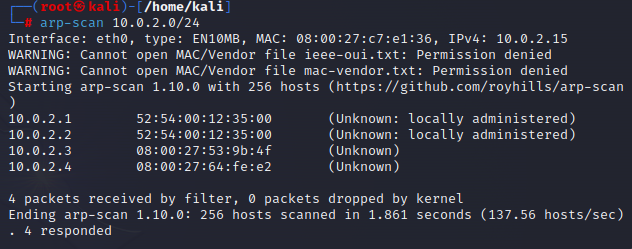
\includegraphics[width=0.8\textwidth]{capitoli/figure/arp-scan.png}
    \caption{Risultato della scansione con \texttt{arp-scan}}
    \label{fig:arp-scan-risultato}
\end{figure}

Anche qui possiamo notare subito un'altra anomalia. Con \texttt{nmap} sono stati rilevati 3 host invece di 2, mentre adesso con \texttt{arp-scan} ne abbiamo rilevati persino 5 (includendo anche la macchina \textbf{Kali} nel conteggio). Osservando con attenzione il risultato, possiamo notare che gli indirizzi \emph{10.0.2.1} e \emph{10.0.2.2} facciano riferimento allo stesso indirizzo MAC (quindi una singola interfaccia con due indirizzi distinti), avvalendo la supposizione precedente che facciano riferimento ad un singolo host interno di \emph{VirtualBox}. A questo punto, se continuiamo a seguire la supposizione che \emph{10.0.2.4} sia l'asset, allora possiamo dire che \emph{10.0.2.3} è un altro host interno di \emph{VirtualBox}. Quindi in realtà gli host attivi non sono 5 come poteva sembrare inzialmente ma sono soltanto 4, e 2 di questi sono host interni di \emph{VirtualBox}.
\subsection{Ulteriore scansione con \texttt{nping}}
A questo punto può sorgere un dubbio, siamo effettivamente sicuri di aver scovato tutti gli host sia "\emph{reali}" che "\emph{fittizi}"? Per essere abbastanza sicuri di averli trovati tutti, evitando così ulteriori sorprese, vale la pena di effettuare un'ulteriore scansione della rete. Per realizzare questa ulteriore scansione è stato utilizzato il tool \texttt{nping}, il quale non fa altro che richiamare il comando \texttt{ping} su tutti gli host forniti in input (quindi ancora una \emph{ping scan}). Per effettuare una scansione con questo tool basta lanciare il seguente comando:

\begin{lstlisting}[language=bash]
    nping -c 1 10.0.2.0/24
\end{lstlisting}

Una volta lanciato il comando otteniamo il seguente output:
\begin{figure}[h]
    \begin{subfigure}{0.5\textwidth}
        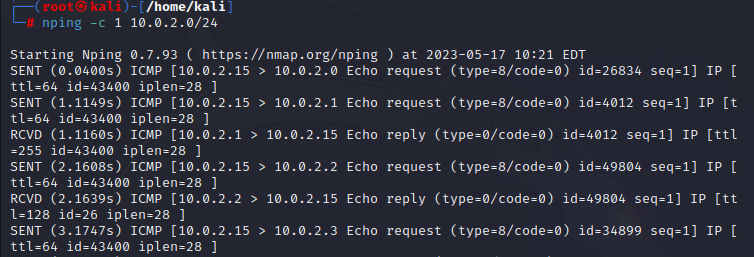
\includegraphics[width=1\textwidth]{capitoli/figure/nping-esecuzione-parziale.png}
        \caption{Esecuzione parziale di \texttt{nping}}
        \label{fig:nping-esecuzione-parziale}
    \end{subfigure}
    \begin{subfigure}{0.5\textwidth}
        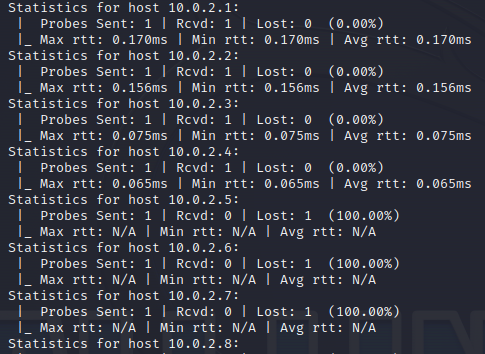
\includegraphics[width=1\textwidth]{capitoli/figure/nping-risultato-parziale.png}
        \caption{Risultato parziale di \texttt{nping}}
        \label{fig:nping-risultato-parziale}
    \end{subfigure}
    \begin{subfigure}{0.9\textwidth}
        \centering
        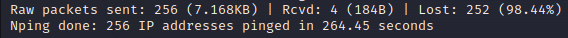
\includegraphics[width=1\textwidth]{capitoli/figure/nping-statistiche.png}
        \caption{Statistiche di \texttt{nping}}
        \label{fig:nping-statistiche}
    \end{subfigure}
    \caption{Output di \texttt{nping}}
\end{figure}

Osservando l'output fornito dal tool \texttt{nping}, sembra che sia conforme con le informazioni ottenute mettendo insieme le precedenti due scansioni. Infatti, possiamo notare dalla Figura \ref{fig:nping-risultato-parziale} che a rispondere al ping sono gli indirizzi \emph{10.0.2.1-4} confermando quindi che sulla rete sono attivi solo 4 host (contando anche la macchina \textbf{Kali}).

\subsection{OS Fingerprinting con \texttt{nmap}}
Con quest'ultima scansione abbiamo terminato di identificare gli host attivi sulla rete e, per questo motivo, possiamo passare al passo successivo. Durante la fase di \emph{Information Gathering} siamo riusciti a stabilire che l'asset è una macchina Linux, ma senza conoscere la versione effettiva del kernel. A tal proposito si può utilizzare ancora una volta il tool \texttt{nmap} che, tramite una tipologia di scansione particolare, è in grado di fare \textbf{OS Fingerprinting} di una determinata macchina presa in input. Per fare ciò, basta eseguire il seguente comando:

\begin{lstlisting}[language=bash]
    nmap -O 10.0.2.4
\end{lstlisting}

Una volta eseguito, l'output ottenuto è il seguente:
\begin{figure}[h]
    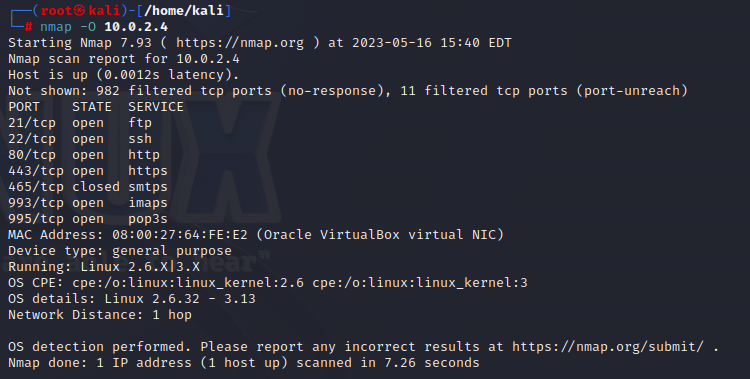
\includegraphics[width=1\textwidth]{capitoli/figure/nmap-os-fingerprint.png}
    \centering
    \caption{Risultato dell'OS Fingerprinting con \texttt{nmap}}
    \label{fig:nmap-os-fingerprint}
\end{figure}

Notiamo che la versione del kernel identificata da \texttt{nmap} risulta essere la \emph{2.6.x/3.x}, in particolare potrebbe trattarsi della versione \emph{2.6.32} o \emph{3.13}. Oltre all'\textbf{OS fingerprint}, possiamo notare che \texttt{nmap} ha eseguito anche una scansione delle porte attive sull'host target. Ovviamente si è limitato solo alle più frequenti (e per questo sarà necessaria una scansione più approfondita nella fase successiva), tuttavia, possiamo notare che ha delle porte aperte che possono essere molto interessanti anche in questo momento. In particolare, le suddette porte sono quelle relative a \textbf{ftp}, \textbf{ssh} e \textbf{http} e, sono particolarmente interessanti poichè si può pensare ad un approfondimento.

\subsection{OS Fingerprint passivo con \texttt{p0f}}
Come accennato in precedenza, grazie a quelle porte aperte si può pensare di fare un'ulteriore scansione ma, questa volta, di tipo passivo. Si può pensare di utilizzare il tool \texttt{p0f}, che si occupa di analizzare il traffico "legittimo" generato da e verso i vari host estrapolando le cosiddette \textbf{Informazioni Caratterizzanti}. Quindi, tutto quello che dobbiamo fare è eseguire il comando \texttt{p0f} e lasciarlo in backround nel mentre che si genera del traffico "legittimo" verso l'asset.

Un primo tentativo che si può fare è quello di generare del traffico \emph{ftp} verso la macchina e, successivamente, controllare se \texttt{p0f} è riuscito ad estrapolare informazioni utili:

\begin{figure}[h]
    \begin{subfigure}{0.5\textwidth}
        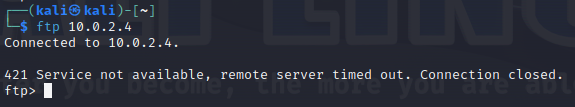
\includegraphics[width=1\textwidth]{capitoli/figure/kali-ftp.png}
        \caption{Generazione di traffico \emph{ftp} legittimo}
        \label{fig:kali-ftp}
    \end{subfigure}
    \begin{subfigure}{0.5\textwidth}
        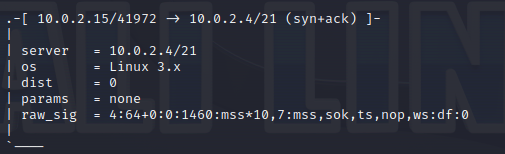
\includegraphics[width=1\textwidth]{capitoli/figure/p0f-ftp.png}
        \caption{Risultato analisi di \texttt{p0f} su traffico \emph{ftp}}
        \label{fig:p0f-ftp}
    \end{subfigure}
\end{figure}

Come si può notare dalla Figura \ref{fig:p0f-ftp}, \texttt{p0f} analizzando il traffico \emph{ftp} è stato in grado di stabilire che il sistema operativo dell'asset ha una versione del kernel \emph{3.x}. Essendo che le tecniche passive non hanno la stessa accuratezza dei metodi attivi (per ovvi motivi), invece di concludere l'analisi con questa informazione è meglio approfondire ulteriormente. A tal proposito, questa volta si è generato del traffico \emph{http} sfruttando il browser \textbf{Mozilla Firefox} installato su \textbf{Kali}. Senza interrompere l'esecuzione di \texttt{p0f}, una volta generato il suddetto traffico è stato ottenuto il seguente output:

\begin{figure}[h]
    \centering
    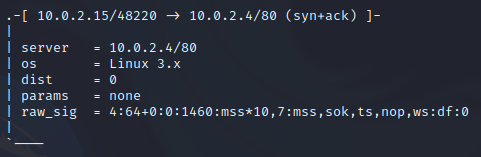
\includegraphics[width=0.7\textwidth]{capitoli/figure/p0f-http.png}
    \caption{Risultato analisi di \texttt{p0f} su traffico \emph{http}}
    \label{fig:p0f-http}
\end{figure}

Consultando anche questo risultato, si può notare che anche qui \texttt{p0f} ha identificato il kernel \emph{3.x}, rendendo più plausibile questa come versione effettiva.

Inoltre, unendo quest'informazione con la scansione attiva realizzata da \texttt{nmap}, è lecito dedurre che molto probabilmente la versione del kernel utilizzata dall'asset sia proprio la versione \emph{3.13}.

\section{Target Enumeration}

%\part{Impatto ambientale}

\backmatter

\end{document}
